\section{Method}
\label{sec:method}
In this chapter we describe the way of how we realized the moody tool. We present the system architecture and explain how we implement the facial and vocal emotion recognition model in more detail.

\subsection{System Architecture}
\label{subsec:method_system_architecture}
The Moody-App is a browser based application written in JavaScript using the React framework\footnote{\url{https://reactjs.org/} (last accessed: 07/23/2021)}. We make use of the AWS platform for data storage and hosting. In particular, we leverage AWS Amplify which covers the whole software lifecycle of mobile- and web applications from development to continuous deployment (CD) and maintenance\footnote{\url{https://aws.amazon.com/amplify/} (last accessed: 07/23/2021)}. Figure~\ref{fig:system_architecture} depicts the high-level system architecture.

\begin{figure}
\centering
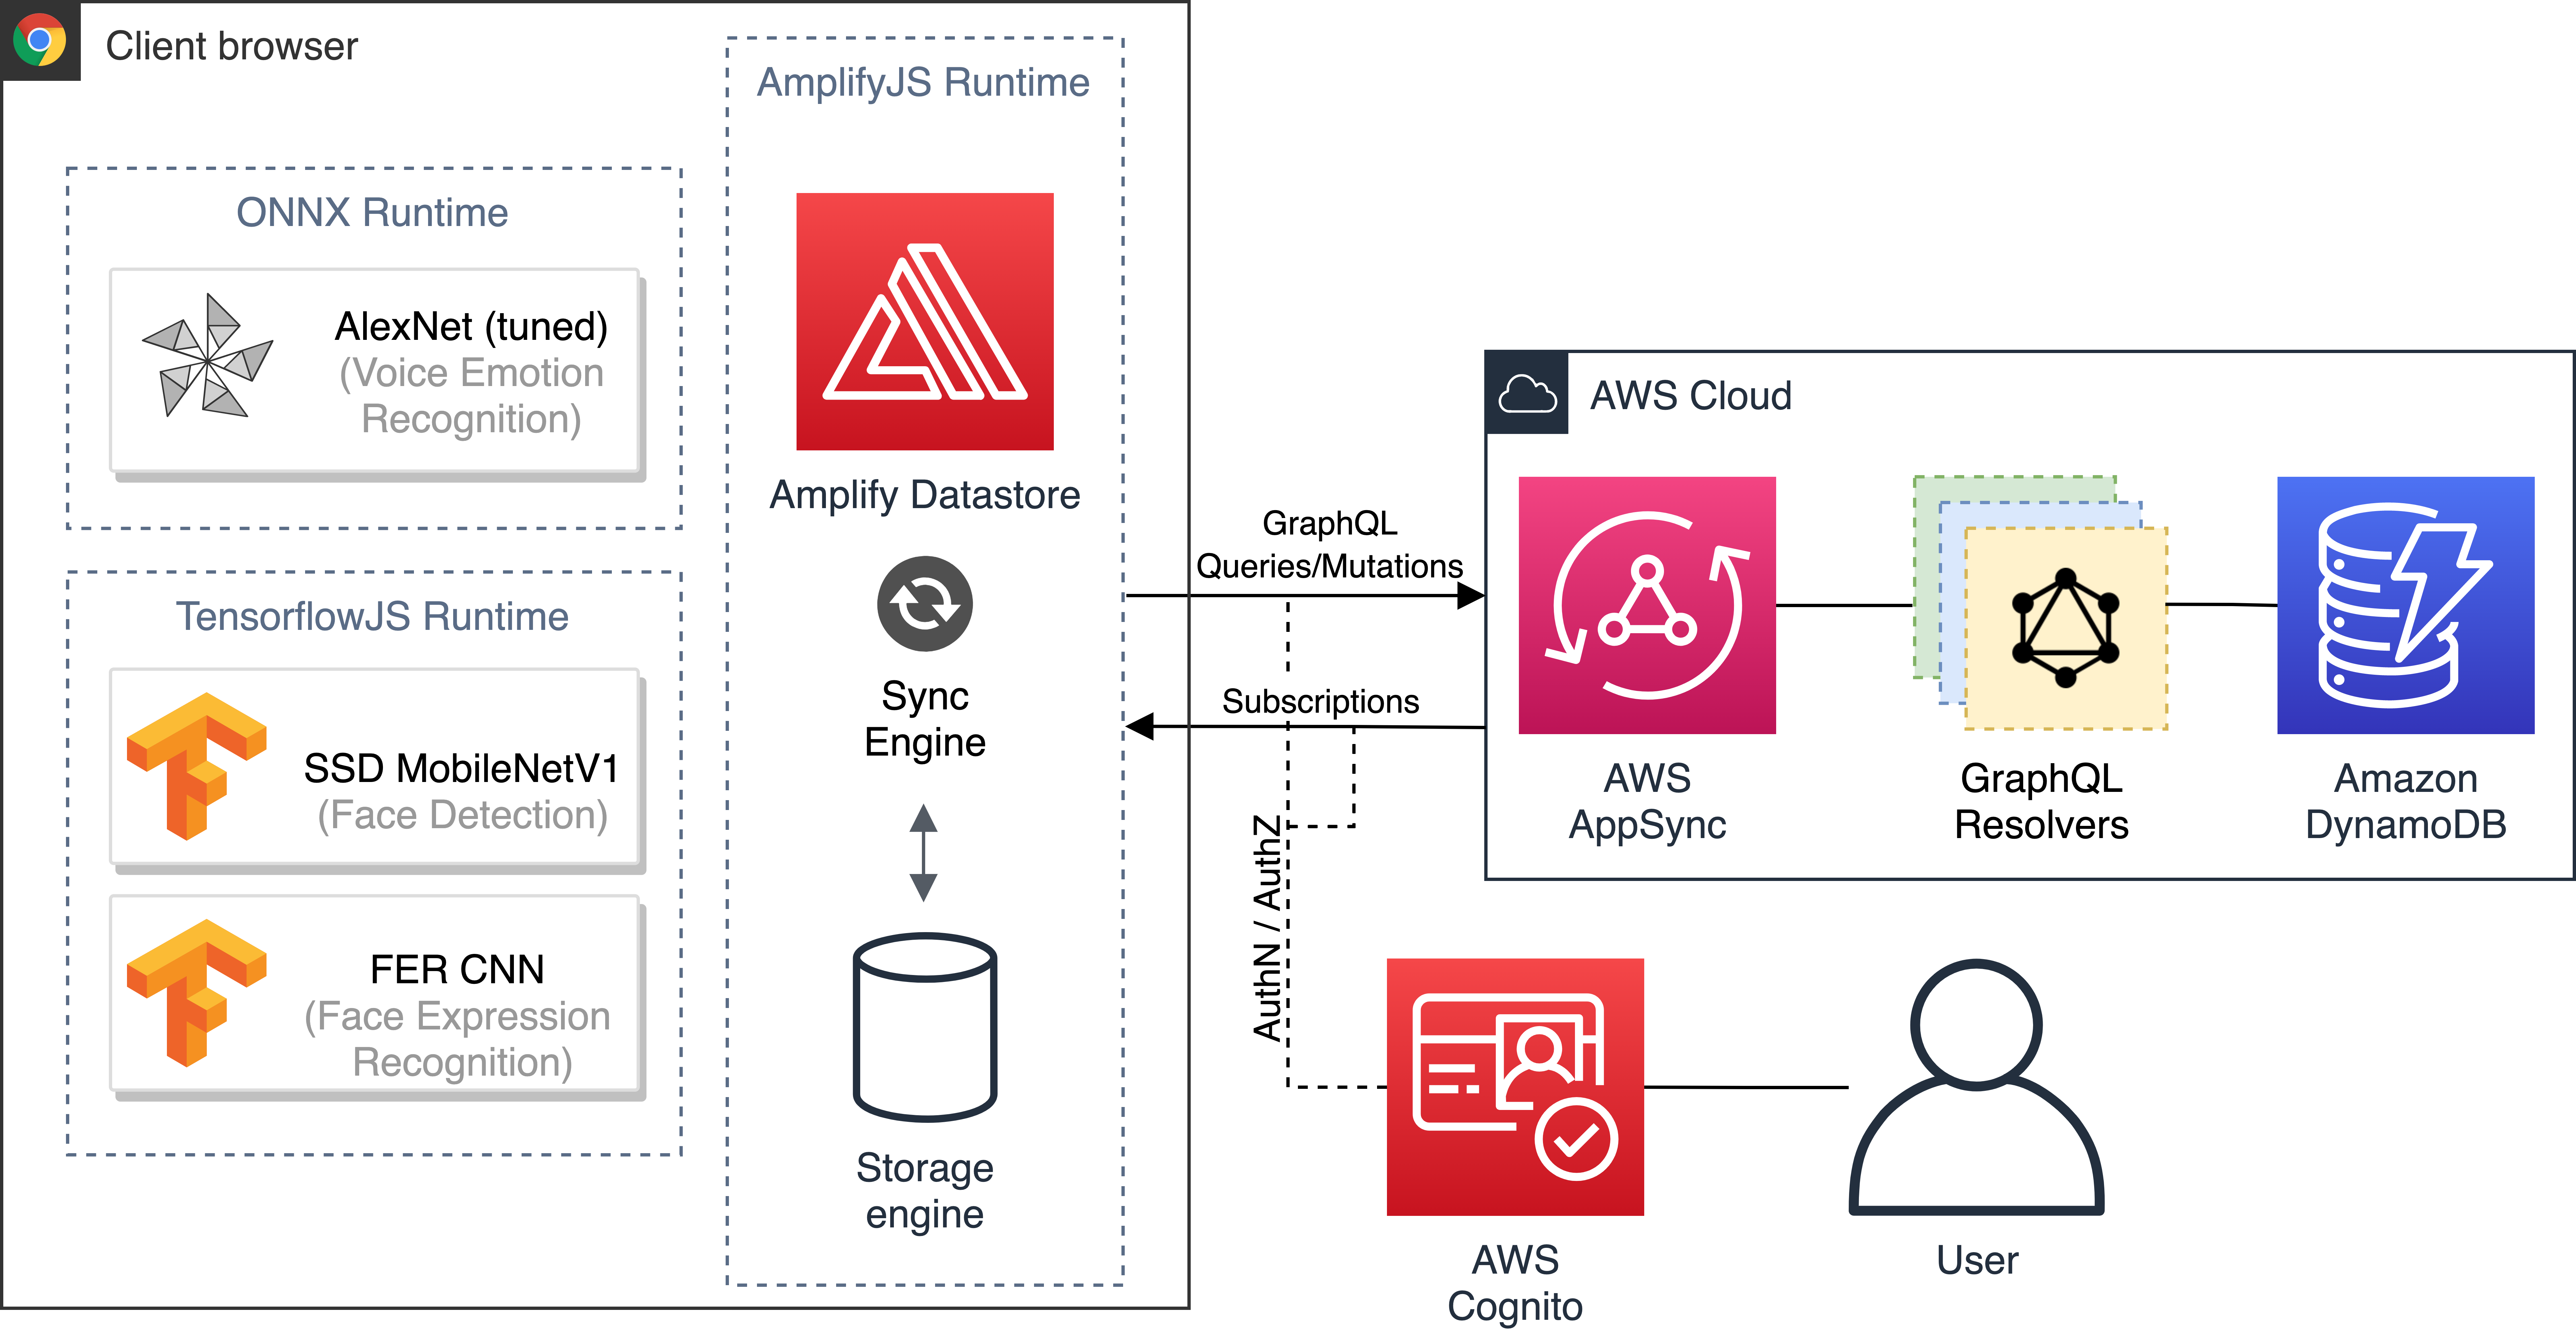
\includegraphics[width=1\textwidth]{assets/system_architecture.png}
\caption{System Architecture Diagram. Moody features a client-server architecture built on top of the AWS platform.}
\label{fig:system_architecture}
\end{figure}

The client side of the application consists of three major subsystems. The first subsystem is AmplifyJS, which is AWS Amplify’s software development kit (SDK) for JavaScript based applications. For us, it provides the means for data modeling, data persistence across devices as well as user authentication and authorization. Our data is modeled according to the third normal form [Quelle]. The full relational schema can be found in Figure~\ref{fig:erd}, Appendix. Amplify Datastore provides an API to a native storage engine which synchronizes asynchronously with the Cloud in the background\footnote{\url{https://docs.amplify.aws/lib/datastore/getting-started/q/platform/js} (last accessed: 07/23/2021)}. The main advantage of this local first approach is a reactive UI because user interaction is decoupled from the network. We keep the UI state consistent across all components using Redux\footnote{\url{https://redux.js.org/} (last accessed: 07/23/2021)} as a state management tool.

The two other subsystems form the machine learning part of Moody. We decided to run all machine learning algorithms locally in the browser of the user. This is beneficial because the internet connection is not impacted by transferring large image and sound data to a remote server every second. In addition, it supports user privacy as only aggregated emotion scores are saved in the Cloud. One drawback is that slower computers might not handle the inference load very well.

The two face models use the TensorflowJS runtime\footnote{\url{https://www.tensorflow.org/js/} (last accessed: 07/23/2021)} and run in a WebGL context\footnote{\url{https://developer.mozilla.org/en-US/docs/Web/API/WebGL_API} (last accessed: 07/23/2021)} allowing for fast computations of the video stream provided by the user. This video stream is captured using the Screen Capture API\footnote{\url{https://developer.mozilla.org/en-US/docs/Web/API/Screen_Capture_API} (last accessed: 07/23/2021)} implemented by all major browsers. As a presenter you typically want to select the window where the faces of your audience are located. Moody will then detect bounding boxes for these faces and perform expression prediction every second giving the presenter feedback. Please note that at the time of writing it is not possible to select a specific window to share in Safari.

Our voice emotion model is originally written in Python with the PyTorch framework\footnote{\url{https://pytorch.org/} (last access: 07/23/2021)}. As it is not possible to run Python code efficiently in the browser we leverage ONNX. ONNX is a standardized open source format to represent neural networks as computation graphs and is currently maintained by the community and Microsoft. It comes along with highly optimized runtimes for different platforms with even better inference performance as compared to the original framework (in our case PyTorch) \cite{developers_onnx_2021}. \texttt{onnxruntime-web}\footnote{\url{https://github.com/microsoft/onnxruntime/tree/master/js/web} (last accessed: 07/23/2021)} is the browser runtime which we use to run the voice emotion model. Since the WebGL backend is not yet feature complete we run our model on the client CPU with WebAssembly\footnote{\url{https://webassembly.org/} (last accessed: 07/23/2021)}. WebAssembly is a compilation target for native languages like C(++) or Rust and allows code execution at close to native speed in the browser. It is currently supported by more than 90\% of all browsers\footnote{\url{https://www.tensorflow.org/js/guide/platform_environment#why_wasm} (last accessed: 07/23/2021)}. To capture the sound of the speaker’s microphone we utilize the Web Audio API\footnote{\url{https://developer.mozilla.org/en-US/docs/Web/API/Web_Audio_API} (last accessed: 07/23/2021)}. As a speaker you are also given the possibility to select the input device. When the voice tracking is active Moody will predict voice emotions every 2.1 seconds and give the speaker live feedback.

All data which is collected from user interaction and the machine learning model predictions is persisted in the AWS Cloud to be available across devices and for further research analysis. Therefore, we have deployed a GraphQL API endpoint with AWS AppSync\footnote{\url{https://aws.amazon.com/appsync/} (last accessed: 07/23/2021)}. This endpoint is called by Amplify Datastore in the background to synchronize new data with the backend. AppSync authorizes each request with AWS Cognito which we use for user authentication. As AppSync is data source agnostic it needs resolvers telling it how to interact with a backend. We chose DynamoDB as the database backend\footnote{\url{https://aws.amazon.com/dynamodb/} (last accessed: 07/23/2021)}. Luckily, Amplify creates these resolvers automatically given a GraphQL compliant data schema\footnote{\url{https://spec.graphql.org/June2018/#sec-Type-System} (last accessed: 07/23/2021)}.

\subsection{Facial Emotion Recognition}
\label{subsec:method_facial_emotion_recognition}
We implement our facial emotion recognition with the “faceapi.js” JavaScript API for face detection, which is implemented itself on top of the tensorflow.js core API and can perform face recognition in the browser. To execute in this project both, the face detection itself and afterwards a linked face expression/emotion recognition, we had to implement two neural networks. The input data are single images from the live videoconference, which are picked up from the meeting tool (e.g. Zoom) window where the participants’ cameras appear. This desktop window has to be selected by the Moody user before he starts the emotion tracking. The two models, which are briefly presented below, were already developed and provided by the authors of faceapi.js, which is why no more data preprocessing was necessary and these only had to be implemented in our system architecture.

First, the algorithm has to detect the faces in the live video and create bounding boxes around the corner points of the faces. For this purpose the face-api.js uses the SSD (Single Shot Multibox Detector) Mobilenet V1 face detection model. The neural net will compute the positions of each face in a picture and return the bounding boxes and their occurrence-probabilities for each face. Instead of then focusing on short inference time, this face detector aims for high accuracy in recognizing face bounding boxes. Nevertheless the size of the quantized model is rather small with about 5.4 MB and thus it works with an acceptable speed. This face detection model has been trained on a dataset called “WIDERFACE” which was developed by the authors Yang et al. (2016) and is a face detection benchmark dataset from publicly available images. The authors chose 32303 images and labeled 393703 faces on these with a high degree of variability in scale, pose and occlusion. The weights for the SSD Mobilenet V1 model and the final face detector, powered by the tensorflow object detection api and trained by WIDERFACE, were provided by yeephycho in a GitHub-Repository.

The second neural net uses the detected faces and their bounding boxes as an input for the face expression recognition model. When all faces were detected on an image, the model receives this information and returns an array consisting of all detected faces and their belonging face expressions. The input images in our tool are single The authors from faceapi.js claim that it is fast and provides reasonable accuracy. The model is about 310kb in size and uses depthwise separable convolutions as well as densely connected blocks. It was trained on a variety of photos, including photographs scraped from the web and images from publicly available sources. Wearing glasses or low light conditions may reduce the accuracy of the forecast results.


\subsection{Vocal Emotion Recognition}
\label{subsec:method_vocal_emotion_recognition}
In the following section, we will explain how we processed our data regarding our voice emotion model, as well how we set the model up and trained it. We used the introduced data sets in the related work chapter, as well as a CNN. 

\subsubsection{Data Preprocessing}
\label{subsubsec:method_vocal_emotion_recognition_data_preprocessing}
The input we will need later for our data model is the waveform of the sound.So for our data preprocessing we then first normalised with RMS normalisation, because the datasets have different volumes. This way we can guarantee that every sound is fed into our model as it really sounds. Because we don't want to fit the dataset specific volume. We use the formula described by Equation \ref{eq:rms_normalization} for this purpose\footnote{\url{https://pydiogment.readthedocs.io/en/latest/_modules/pydiogment/auga.html#normalize} (last accessed: 07/23/2021)}:
\begin{equation}
\label{eq:rms_normalization}
y_n=\sqrt{\frac{N-10\,(\frac{r}{20})}{\sum_{i=0}^{N-1}{x_i^2}}}\cdot{}x_n
\end{equation}

\subsubsection{AlexNet Architecture}
\label{subsubsec:method_vocal_emotion_recognition_alexnet_architecture}
The Mel Spectrogram then runs on the actual CNN. Together with the freely available and augmented data sets we trained our CNN. We have tried out two different well-known models. One is AlexNet and the other is ResNet18. The performance of both models was almost identical, only the size of the models differed. Since the Alexnet with 32.3 MB is almost half the size of the ResNet18 with 59.7 MB, and has fewer parameters, we decided to use the AlexNet for our web app. This is then exported to ONNX to be executed in the browser with the help of ONNX runtime-web for inference.The voice emotions are recorded in time windows of 2.1 seconds. This time is the average duration of the samples in the data sets we use.
